\chapter{\label{detchar}Detector Characterisation with SOAP}
%%%%%%%%%%%%
%%%%%%%%%%%%
%%%%%%%%%%%%
%%%%%

When searching for \gls{GW} signals, it is important to understand the origins
of noise artefacts in the detector data which does~\chris{do} not originate from an
astrophysical source.  A large fraction of \gls{GW} search algorithms,
including SOAP above~\chris{above?}, assume that the detectors noise follows a Gaussian
distribution~\chris{we don't totally assume that, e.g., the line aware stat you
have already discussed}.  However, the detectors contain artefacts which do not follow
this distribution.  These artefacts can negatively affect many searches for
\glspl{GW} as they can be easily mistaken for a real \gls{GW} signal.  Some of
the potential sources of these artefacts have been mentioned in
Sec.~\ref{intro:detector:noise}.  There are many different classes of artefact,
including: glitches, which are short duration broad band bursts in
power~\chris{comma} and
instrumental lines, which are long duration narrow-band signals.  To conduct a
reliable search there are two main tasks which are necessary for detector
characterisation.  The first is identifying the artefact such that any search
knows which frequency bands and time segments are contaminated.  The search can
then address that section of data, this could mean removing that section of
data or use~\chris{using} more sophisticated techniques to deal with the artefact
\citep{pankow2018MitigationInstrumental}.  The second task is to find the
source of the artefact~\chris{be clearer. You mean the particular instrumental
or environmental source}.  If the source of the artefact is found, it can
potentially be removed or limited for future data runs.

The focus of this chapter is on instrumental lines and how they affect \gls{CW}
searches~\chris{isn't it more about how to search for and identify intrumental
lines?}.
Sec.~\ref{detchar:lines} will introduce different sub-classes of instrumental line and how each of them affects a \gls{CW} search.
Sec.~\ref{detchar:monitor} will outline how these artefacts are detected and monitored, and describe current tools used for this task.
Sec.~\ref{detchar:soap} will describe how the \gls{CW} search algorithm
introduced in Sec.~\ref{soap} can be used to search for instrumental lines.
Finally Sec.~\ref{detchar:summary} will show the outputs of the search and this
is displayed for ease of use~\chris{final sentence is a grammatical mess}.



%%%%%%%%%
%%%%%%%%%%
\section{\label{detchar:lines}Instrumental lines}
%%%%%%%%%
%%%%%%%%%

%
% Introduce instrumental lines

Instrumental lines have the general structure that they are persistent noise
artefacts~\chris{this isn't really a structure}.  There are many classes of
instrumental line spanning a range from narrow, fixed frequency spectral
artefacts to broader ($<0.1$ Hz) features which have a time varying frequency
known as wandering lines.  For many of these lines, it is difficult to
distinguish them from an astrophysical signal.  They affect search methods in
two main ways.  They can cause the search to produce outliers which are then
considered as \gls{GW} candidates.  Extra efforts then have to be made to
analyse these outliers further.  If the line is close to the \gls{GW} signal in
frequency, then it can conceal the power of the \gls{GW}, or if it is
overlapping, the search becomes very difficult~\chris{how exactly?}.  It is therefore crucial to
understand the structure and origin of these lines when performing a search for
\gls{GW}, specifically \gls{CW} and stochastic searches \joe{explain why
stochastic}.~\chris{lines also affect the noise floor estimate and can
therefore contaminate searches indirectly.}

%
% What lines look like and how the appear in the GW channel

Some instrumental lines are clearly visible when looking at a \gls{ASD} or
\gls{PSD} of the \gls{LIGO} detectors. Figure \ref{detchar:line:psd} shows the
\gls{ASD} for \glspl{LIGO} Hanford and Livingston detectors during their first
observing run (O1) \citep{GWOpen}. This clearly shows some peaks which are
associated with strong lines, some have been labelled~\chris{strange use of
comma here}. There are however, many
more weaker lines which become visible when spectra are averaged over longer
times.
%
\begin{figure} \centering
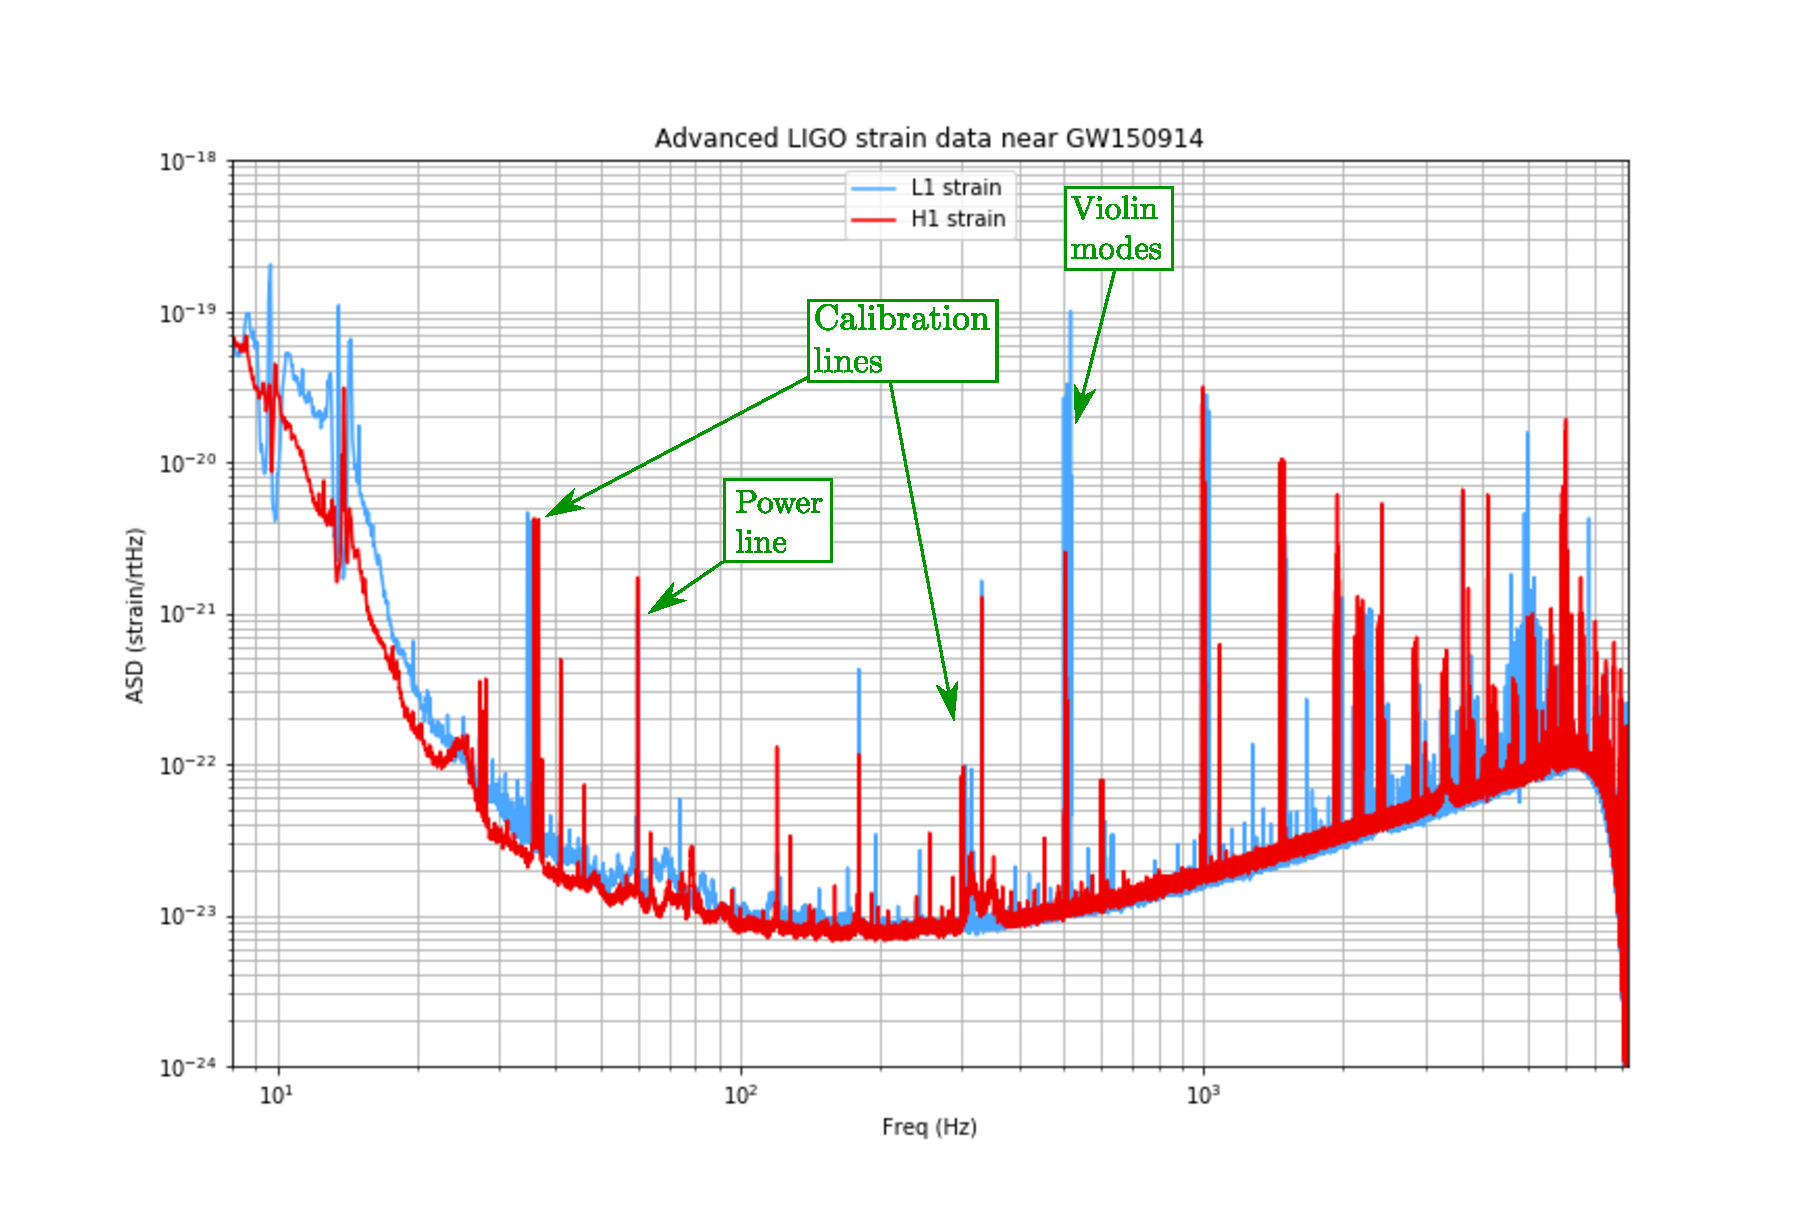
\includegraphics[width=\textwidth]{C5_detchar/ligo_o1_asd_annot.pdf}
\caption[Strain \gls{ASD} for the \gls{LIGO} detectors.]{There are many
features in the \gls{LIGO} detectors averaged \gls{ASD}.~\chris{start every
figure cpation with a 1 sentence summary/description/title. In this case you
are plottin the LIGO detector ASDs at the time of the GW150914 event in O1.
Also, I would personally cut out the title and maybe mention the dodgy drop at
the high frequencies.} This image was taken
from \citep{GWOpen} where I have~\chris{maybe best to not use language like
this. Better to say that certain lines have been annoted rather than state "I"} annotated some of the stronger lines. The
power line from the mains in the USA is at 60 Hz. Some of the calibration lines
are around 30 Hz, 331 Hz and 1083 Hz. The various violin modes of the
suspensions are at 300, 500, 600 and 900 Hz where I have only marked the 500 Hz
mirror suspension modes \citep{GWOpen}.} \label{detchar:line:psd} \end{figure}
%
The \gls{ASD} in Fig.~\ref{detchar:line:psd} shows the time averaged spectra
~\chris{of} the \gls{GW} channel of the \gls{LIGO} detectors.  The \gls{GW} channel is the
error signal on the mirrors whilst they are being held on a resonance, i.e. how
much the mirrors have to be moved to keep the same intensity at the output of
the interferometer.~\chris{this last statement seems out of place and would be
better used in the introduction chapters - after being expanded upon a bit. The
error signal in this case is just $h(t)$ which you have been quite happy to use
without this kind of description until now.}  The lines seen in the spectrum are not from any \gls{GW}
and are usually from ground based sources.  To see the lines in the \gls{GW}
channel, they must be coupled in via some mechanism~\chris{the average reader
won't know exactly what you mean by "coupling in". What does it mean?}.  There are a number of
ways in which this happens which are outlined in
\citep{covas2018IdentificationMitigation}.  This includes coupling via shared
power and grounds~\chris{power and grounds? Add some extra helpful descriptive
words for the reader. What is "grounds"?}.  When different components share the same power supplies, if
a component draws power with a given period, then the voltage will decrease
repeatedly at this frequency.  Another component which shares this same power
supply can then also see this drop in voltage and this can potentially become
visible in a recorded output.  Another mechanism is coupling through magnetic
fields, this is common when cables are close to each other, the magnetic field
in one can affect the other, therefore, coupling noise between different
systems.  Coupling can also occur though a physical connection, known as
mechanical coupling, for example the resonances of the suspension fibers which
couple directly into the mirrors~\chris{and therefore the output error signal?}.

%
% Origins of some lines and how they can be mitigated

Many of the spectral lines seen in the frequency spectrum,
Fig.~\ref{detchar:line:psd} are fundamental to the design of the detector.
These cannot~\chris{never say never - don't be so definitive.} be eliminated, therefore need to be understood such that their
effect on searches is minimised.  Some of the strongest of these lines are
listed below:

\begin{description}
	\item[Power line] The power line harmonics are fundamental to the
detector and originate from the mains~\chris{power} supply in the
USA~\chris{acronym?}. These lines exist at 60 Hz which is the frequency of the
mains alternating current \citep{aasi2015CharacterizationLIGO}. \chris{The} European
detectors Virgo and GEO have a power line at 50 Hz instead of 60 Hz.
	
        \item[Violin modes] The violin modes are associated with the
suspensions~\chris{} of the mirrors and the beam splitter in the detector. These are
designed to have a narrow frequency spectrum such that they contaminate as
small a part of the spectrum as possible. These are the lines around 500 Hz for
the mirrors and 300, 600 and 900 Hz for the beam-splitter \citep{GWOpen} in
Fig.~\ref{detchar:line:psd}.
	
        \item[Calibration lines] The mirrors of the \gls{LIGO}
detectors,~\chris{random misplaced comma} are
held at a resonance~\chris{what does this mean? Every time you say something
vague like this you are begging the external examiner to question you about it.
Do you want to be questioned about the resonance of cavities?} of the cavity in the arms of the interferometer. This then
requires a feedback loop to hold them at resonance as a \gls{GW} passes the
detector. Calibration lines are used to calibrate this feedback loop such that
the arm length changes are accurate
\citep{tuyenbayev2016ImprovingLIGO,coughlin2010NoiseLine}.~\chris{yes, but what
is a calibration line? You say that they are used for something but what are
they?}  
\end{description}
In \citep{davis2019ImprovingSensitivity}, techniques are used to counter the
affect of power lines and calibration lines on searches~\chris{this sentence
seems to come out of nowhere and stand in isolation}. 

Along with~\chris{an example of slightly less formal writing here. Along could
be replaced by Together.} the fundamental lines of the detector which
cannot~\chris{never say never. My Mum would have never belived you could cook
rice in less than 15 minutes but I can do it in the microwave in 1 minute 30.} be
removed at the source, there are a large number of other lines whose source has
been found and can be removed.  Many of these are from mechanisms described
earlier such as shared power supplies or grounds. These can be removed by, for
example, using a different power supply for different systems. See
\citep{covas2018IdentificationMitigation} for a full investigation into the
mitigation of these lines.

%
% How lines affect CW searches

These lines have~\chris{a} large effect on all searches for \glspl{GW} both if
the astrophysical signals frequencies overlap with the frequency of the line
and can cause outliers~\chris{need some extra punctuation to understand this
sentence}.  Long duration searches for \glspl{CW}~\chris{Isn't it search for
long duration CWs? Your way simply says that the searches themselves are long
duration} are
particularity sensitive to this type of artefact.  As described in
Sec.~\ref{searchcw}, \glspl{CW} are long duration signals with a slowly varying
frequency.  In the case of an isolated neutron star, the signal which is
searched for is narrow-band and a fixed frequency which~\chris{and not which} is Doppler modulated by
the earths rotation and orbit~\chris{also amplitude modulated by the antenna
patterns as Earth rotates}. For certain areas of parameter space, such as
close to the poles~\chris{what are the poles?}, the astrophysical signal of an isolated neutron star can
appear very similar to a narrow band fixed frequency instrumental line.  Many
of these lines~\chris{the effects of these lines} can be mitigated by using multiple detector data. If a signal
appears in one detector and not the others, then it is likely that the signal
is from an instrumental line and not an astrophysical source.  These
contaminated frequency bands can either be removed or a statistic similar to
that described in Sec.~\ref{soap:las} or \citep{keitel2014SearchContinuous} can
be used to limit their effect.  However, there are many examples of
instrumental line which appear at the same or similar frequencies in multiple
detectors.  These pose a real challenge to some \gls{CW} searches, and require
a lot~\chris{again, not very formal. a lot could be substantial or an in-depth
etc.} of investigation to limit their affect.

%%%%%%%%%%
%%%%%%%%%%
\section{\label{detchar:monitor}Identifying and monitoring instrumental lines}
%%%%%%%%%%
%%%%%%%%%%
\joe{mention wiki page somewhere, eg : https://wiki.ligo.org/CW/O3aLineCleaningInfo}
%
% into to why lines are monitored

When a detector is running, it is very important to identify instrumental lines
and monitor them.  This can then lead to either locating the origin of the line
such that it can be removed, or allowing it to be flagged for other search
algorithms.  The lines affect searches in the \gls{GW} channel, this is the
output of the detector~\chris{in} which \gls{GW} are observed and is the data used is
previous chapters.  This is the channel where the affect of lines is intended
to be minimised.~\chris{this paragrpah could be tidied up a bit. Very clunky.}

%
% Auxiliary channels 
As well as~\chris{Formal: In addition to} the \gls{GW} channel, the detector
records many different channels known as auxiliary channels.  These channels
monitor many components of the detector, and importantly are not sensitive to
\glspl{GW}.  Many of the channels useful for line searches are the \glspl{PEM}.
These include sensors~\chris{do the channels include sensors? No. The sensors
are used to record the data assigned as "channels". Be careful with language.}
such as seismometers measuring the ground motion, temperature sensors,
magnetometers etc.  These channels can be very useful in identifying the source
of an instrumental line.  The main goal is to reduce the number of artefacts in
the \gls{GW} such that it is as close to Gaussian noise as possible.  If an
artefact shows up in the \gls{GW} channel in coincidence with one of the
\gls{PEM} then this is an indicator that the artefact originates from something
related to that \gls{PEM}.  For example, say a~\chris{too informal - consider
that a} magnetometer located near some~\chris{too informal}
electronics has a long duration line in its spectrum at the same frequency as
the main \gls{GW} channel.  This indicates that noise from this piece of
electronics is somehow coupling into the detector.  One can then investigate
that piece of electronics further to see~\chris{informal - test or investigate} how it couples in.

%
% tools to monitor all the channels

There are a number of tools which are used to monitor these spectral lines,
along with a team of people which~\chris{that} regularly look though the
results,~\chris{not a comma situation in this sentence} a summary
of these for the first two observing runs of \gls{LIGO} can be found in
\citep{covas2018IdentificationMitigation}.  Some of the tools used are
described below.~\chris{sort out the grammar in this paragraph} 

\begin{description}
        \item[Fscan] Fscan~\chris{Double Fscan} \citep{coughlin2010NoiseLine}
takes \glspl{FFT} of the raw detector data, typically these are 1800s long.
This is done for all of the auxiliary channels as well as the \gls{GW} channel.
The \glspl{FFT} are then averaged over a day and time-frequency spectrograms
are generated. After known lines such as Violin modes and power lines are
subtracted, noise lines can be identified. A threshold can be set and
anything~\chris{informal}
in the spectrograms which exceed this threshold are~\chris{is} flagged as a line. These
can then be compared across multiple different channels. More detail on how the
lines are identified can be found in \citep{coughlin2010NoiseLine}.
	
        \item[Coherence] Coherence~\chris{Double Coherence} searches for the coherence between different
channels and different detectors. This is similar to searches for stochastic
gravitational waves. More detail of how this works can be found in
\citep{covas2018IdentificationMitigation}.~\chris{You could potentially expand
upon this and give a few more details.}
	
        \item[Finetooth] Many of the instrumental lines found are part of
combs. These are repeating structures where the harmonics (teeth) of a
line~\chris{So the terminology is mixed up here. A signal that exhibits some
kind of periodic frequency or amplitude modulation can appear as distinct
harmonics - each of which is a line. The collection of regularly spaces lines
make up the "comb". }
make up the comb which is defined by the start frequency and tooth spacing.
Finetooth is a tool which identifies and monitors these combs
\citep{neunzertDailyComb}.
	
        \item[NoEMi] NoEMi~\chris{Double NoEMi} uses \glspl{FFT} and identifies peaks within the
spectrum. It can then find coincidences with auxiliary channels and label is
there are overlapping peaks with the \gls{GW} channel~\chris{grammatical
badness in this sentence}. This can then tracks the
lines with time~\chris{obvious typo but also an unusually short sentence}. All of the information is stored in a database where more
detail on its operation can be found in \citep{accadia2012NoEMiNoise}.~\chris{I
am not really left with any clear understanding of how this works. In general,
you have an opportunity here to at least double the text alloacted to each of
these competing/complimentary line finding approaches.}
	
\end{description}


These tools offer many ways for the detector characterisation team~\chris{it
seems strange to be limiting the use of these tools (and your own) to a
specific group of people. I would suggest that you don't refer to the detchar
team but rather refer to GW scientists working on understanding the behaviour
of the detector} to identify
instrumental lines and hunt for their source. A summary of these efforts for
the advanced \gls{LIGO} data can be found in
\citep{covas2018IdentificationMitigation}, or the \gls{LIGO} wiki page {\tt
\url{https://wiki.ligo.org/DetChar/O3LinesCombsInvestigations}}~\chris{this
link is specific to O3 and not to the advanced detectors in general}. The following
sections describe how the SOAP search described in Sec.~\ref{soap} can be used
as an extra tool to aid in the identification and monitoring of instrumental
lines.

\clearpage

%%%%%%%%%%%
%%%%%%%%%%%
\section{\label{detchar:soap}Identifying and cleaning lines with SOAP}
%%%%%%%%%%%
%%%%%%%%%%%%

% Why SOAP may be good at finding instrumental lines
% 
The SOAP search has been run on a number of observing runs to search for \gls{CW}. 
One of the major factors which limited the sensitivity of the search is the presence of instrumental lines within the data. 
Many of the potential candidates which SOAP returned could be identified as an instrumental lines 
An example of once of these candidates can be seen in Fig.~\ref{detchar:soap:astrowander}.
%
\begin{figure}[h]
	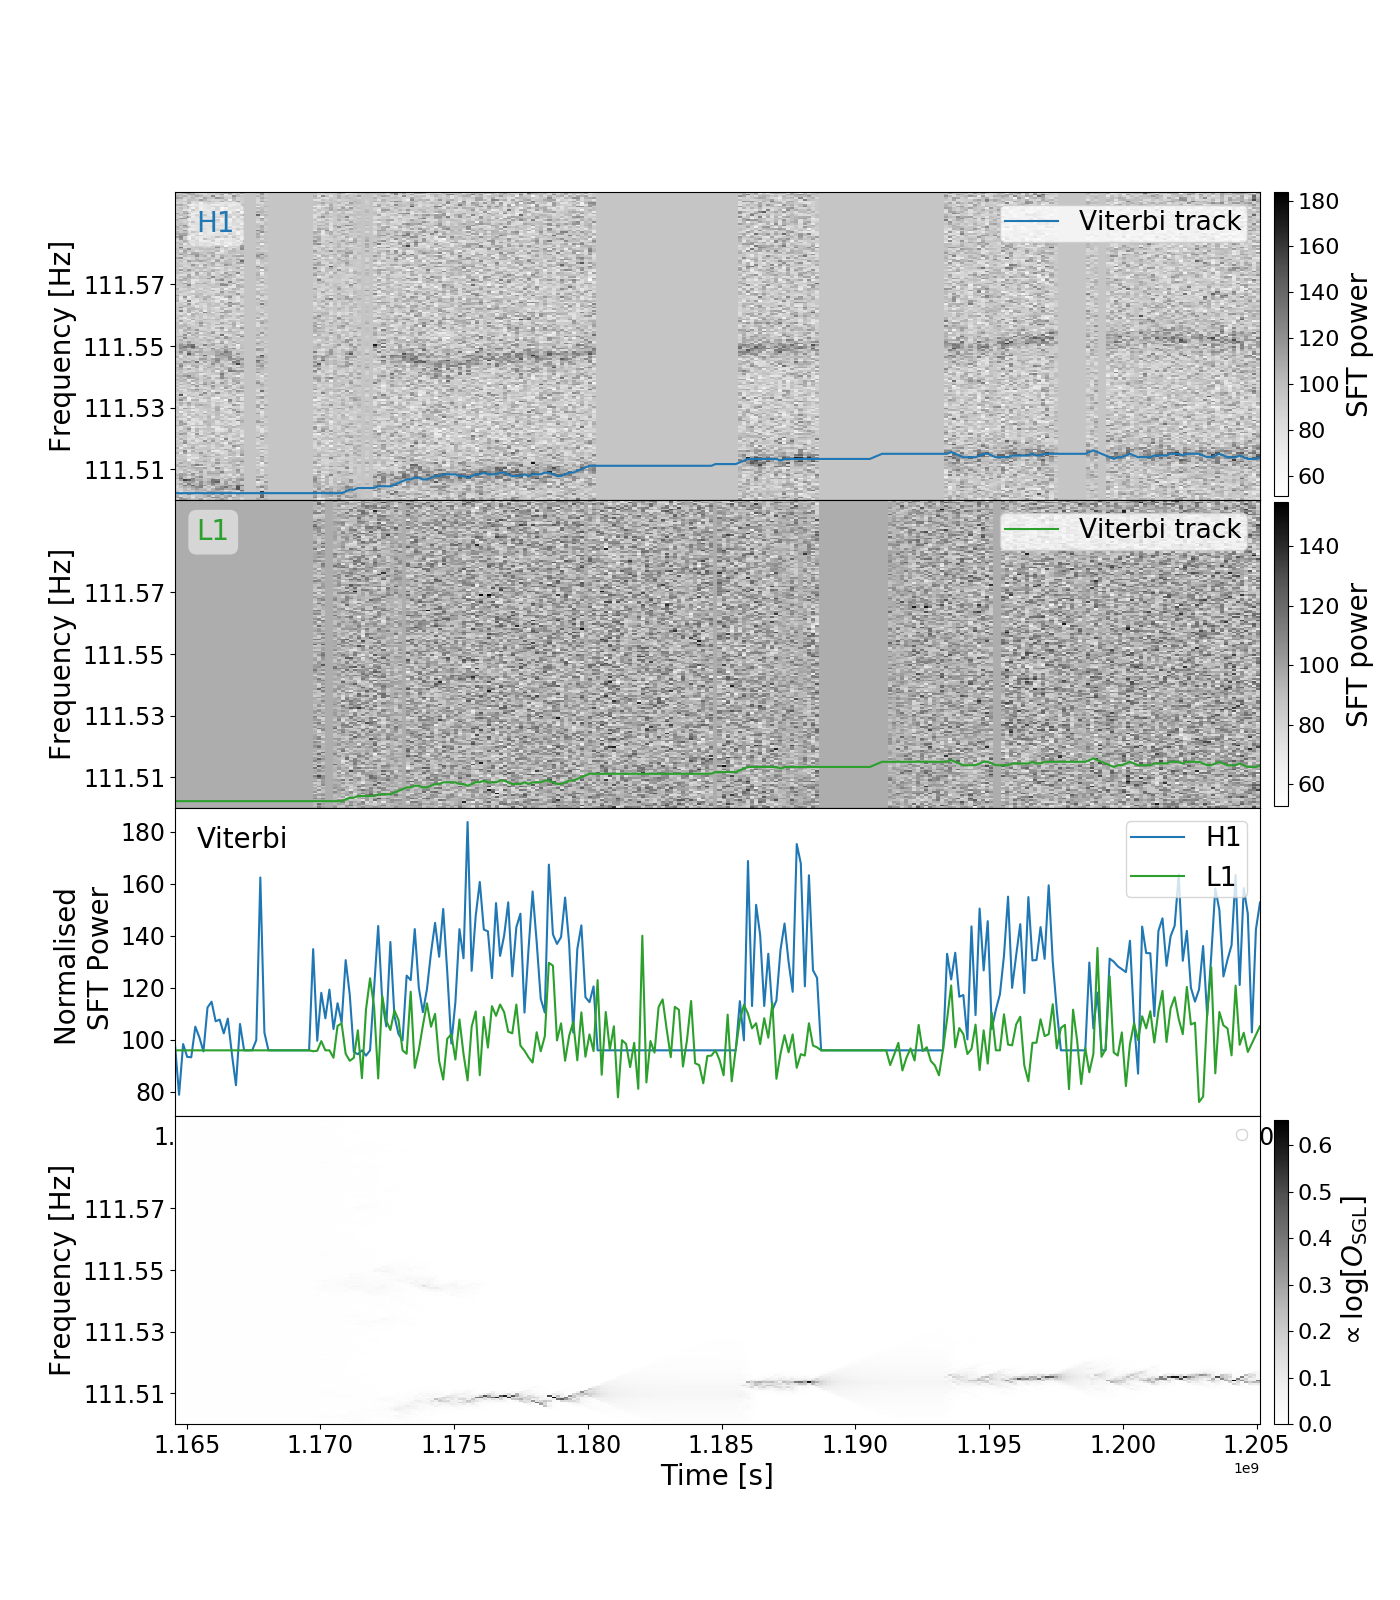
\includegraphics[width=\textwidth]{C5_detchar/plot_F111_5_wandering_line.png}
	\caption[Broad wandering line example.]{Broader instrumental lines are generally weaker and can be mistaken for an astrophysical signal by the SOAP astrophysical search. Above an example of two broad line in the H1 detector is shown, where SOAP has identified one of the. The top two panels show the summed spectrograms from the H1 and L1 panels with the optimal Viterbi track overlaid. The third panel shows the normalised spectrogram power along the Viterbi track for each of the detectors. The final panel shows the Viterbi map for this frequency band.}
	\label{detchar:soap:astrowander}
\end{figure}
%
Figure \ref{detchar:soap:astrowander} shows a broad and wandering line in a single detector causing the SOAP search to mistake it for an astrophysical signal. 
This is because the SOAP line aware statistic from Sec.~\ref{soap:las} find areas of higher power which are consistent between detectors according to the parameters of the statistic. 
These types of line are difficult to mitigate in the astrophysical search, however, this has a side effect of being useful to identify the instrumental lines themselves.
In this section, I will explain the setup of the search to identify instrumental lines.

Whilst it is useful to run searches on auxiliary channels when trying to identify the lines source, the aim of this search was to flag potential lines.
Therefore, this search currently only runs on the \gls{GW} channel where they flagged lines can be investigated further.
In the future this could be modified to search multiple channels to find coincidences between them. 
Sec.~\ref{soap} described how multiple detectors can be used to increase the sensitivity of a search for \glspl{CW}. 
However, when searching for instrumental lines, the aim is to have the reverse effect, therefore, a simple search is run separately on each detector. 
This then removed any of the statistics developed in Sec.~\ref{soap:las} and uses the `normalised' \gls{SFT} power as the statistic in the SOAP search.
The single detector search then has one parameter to vary, the transition matrix parameter. 
This governs how probable the frequency track is to transition up straight or down a frequency bin.
In this search we are aiming to find any non Gaussian artefacts, therefore, we allow an equal probability for the track to jump in any direction, however, limit it to change by one frequency bin after each time segment.  
Whilst the astrophysical search summed the \glspl{SFT} over one day as shown in Fig.~\ref{detchar:soap:astrowander}, for the line search, we assume that instrumental lines are stronger than astrophysical signals and therefore should be identifiable in the raw 1800s long \glspl{SFT}.
The Fscan search described above generates \glspl{SFT} every day of varying lengths, this include 1800 s long \glspl{FFT}. 
For this line search, we split the 1800 s long Fscan \glspl{FFT} into 0.2 Hz wide sub-bands and run the single detector search on each sub-band. 
This then returns the same outputs as described in Sec.~\ref{soap} and Sec.~\ref{machine}: the frequency track (Viterbi track), a Viterbi map and a Viterbi statistic. 
Here the Viterbi statistic is just the sum of the \gls{SFT} power along the frequency track. 
The line search then outputs plots as shown in Fig.~\ref{detchar:soap:linewander}, \ref{detchar:soap:noiseplot}, \ref{detchar:soap:lineplot} and \ref{detchar:soap:wanderplot}. 
These plots and the equivalent plots for other sub-bands can then allow each sub-band to be classified into containing an instrumental artefact or not.
An example of the SOAP line search being run on the H1 detector on the same instrumental line but with slightly wider frequency band as Fig.~\ref{detchar:soap:astrowander} can be seen in Fig.~\ref{detchar:soap:linewander}
This shows how the line search identifies the same instrumental line albeit at a higher resolution and can flag it for further investigation.
%
\begin{figure}
	\centering
	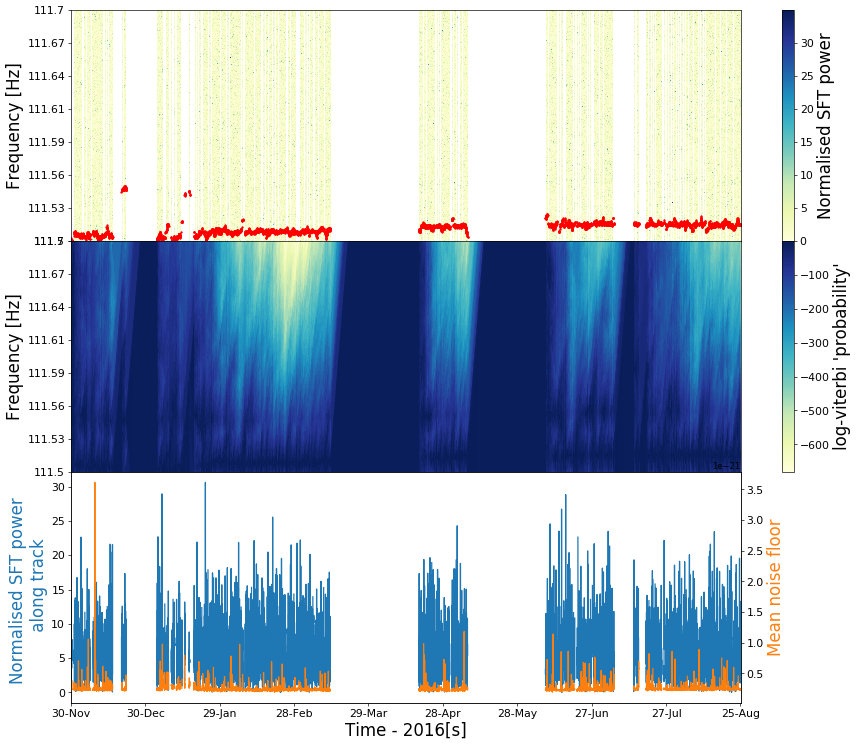
\includegraphics[width=\textwidth]{C5_detchar/track_F111_5_111_7_wander_2.png}
	\caption[Example SOAP output for wandering line]{The SOAP line search is run on a similar frequency band to Fig.~\ref{detchar:soap:astrowander}. This returns a similar track however at a resolution of 1800 s rather than one day.}
	\label{detchar:soap:linewander}
\end{figure}
%

\begin{figure}
	\centering
	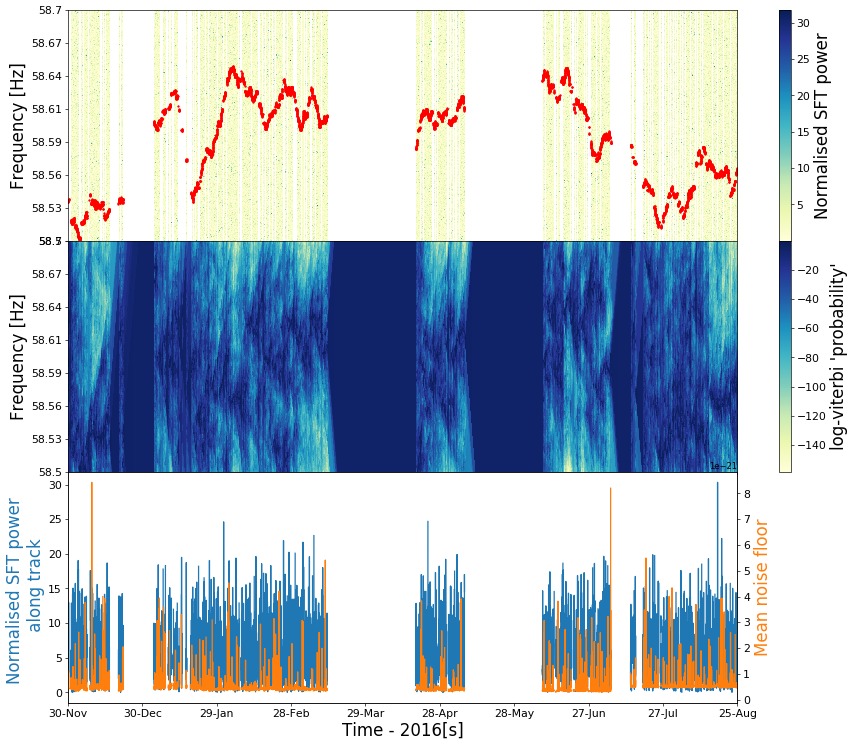
\includegraphics[width=\textwidth]{C5_detchar/track_F58_5_58_7_noise.png}
	\caption[Example SOAP output for Gaussian like noise.]{The SOAP search outputs three main quantities, the Viterbi maps, the Viterbi track and the Viterbi statistic. The Viterbi track is shown above overlaid onto the 1800s \gls{SFT} power spectrum including the detector gaps for \glspl{LIGO} Hanford detector (H1) in its second observing run (O2) \citep{}. This track is an indicator as to what type of signal the track is following. The above track indicated that this is just noise. The returned Viterbi statistic is also consistent with that of noise. The Viterbi map is another visualisation of the sub-band, how to interpret this has been explained in previous sections. However, here there does no appear to be a clear signal. The final panel is a way to visualise how the \gls{SFT} power changes along the Viterbi track. Also on this plot is an estimate of the mean noise floor for this band to visualise how the sensitivity of the detector changed over the course of the run. }
	\label{detchar:soap:noiseplot}
\end{figure}
%
Fig.~\ref{detchar:soap:noiseplot} shows an example of the spectrogram of a sub-band which does not contain any signal or spectral artefacts but is Gaussian distributed noise. 
The track in the top panel of this plots shows the power spectrum including detector gaps from 1800 s \glspl{SFT} in \gls{LIGO} Hanford's data from its second observing run (O2). 
The Viterbi track is overlaid and the structure of the track indicates that there is no signal present, this is because the track appears to be randomly wandering and has a large spread over the entire band. 
The Viterbi map plot does not show much structure and contains areas of low log-probability.
Using this information along with the Viterbi statistic result, this particular sub-band can be considered to not contain an instrumental artefact. 
%
\begin{figure}
	\centering
	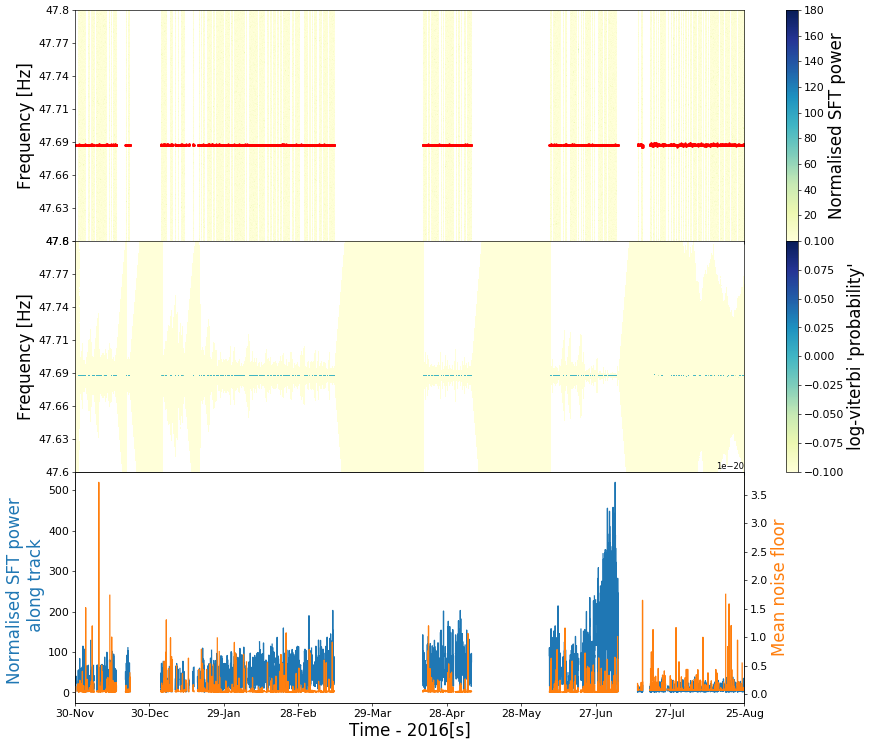
\includegraphics[width=\textwidth]{C5_detchar/track_F47_6_47_8_linenarrow.png}
	\caption[Example SOAP output for string narrow instrumental line.]{The equivalent plot as in Fig.~\ref{detchar:soap:noiseplot} can be made when there is a narrow spectral artefact in the band. The above is again results from \glspl{LIGO} Hanford detector (H1) in its second observing run (O2) using 1800s \gls{SFT} power spectrum. In this there is a narrow spectral line at $\sim 47.69$ Hz. The Viterbi track then follows this line of high power. The Viterbi map has much higher values for the log-probability in this line case compared to the noise case, this is an indicator some real signal. The probability in the Viterbi maps drops to zero in some areas due to the strength of the instrumental line. }
	\label{detchar:soap:lineplot}
\end{figure}
%

Fig.~\ref{detchar:soap:lineplot} demonstrates the same figure as before but now with a strong and narrow instrumental line in the sub-band. 
The Viterbi track now clearly indicates that there is a narrow spectral artefact present in the sub-band. The track does not have much spread over the band and stays at an approximately fixed frequency. 
The Viterbi map plot then shows that there are clear areas around the track which are of high log-probability. 
The areas of white in the Viterbi maps area areas where the probability of a signal falls to zero. 
These pieces of information along with the large value of the Viterbi statistic indicate that there is a narrow spectral artefact within the sub-band. 
%
\begin{figure}
	\centering
	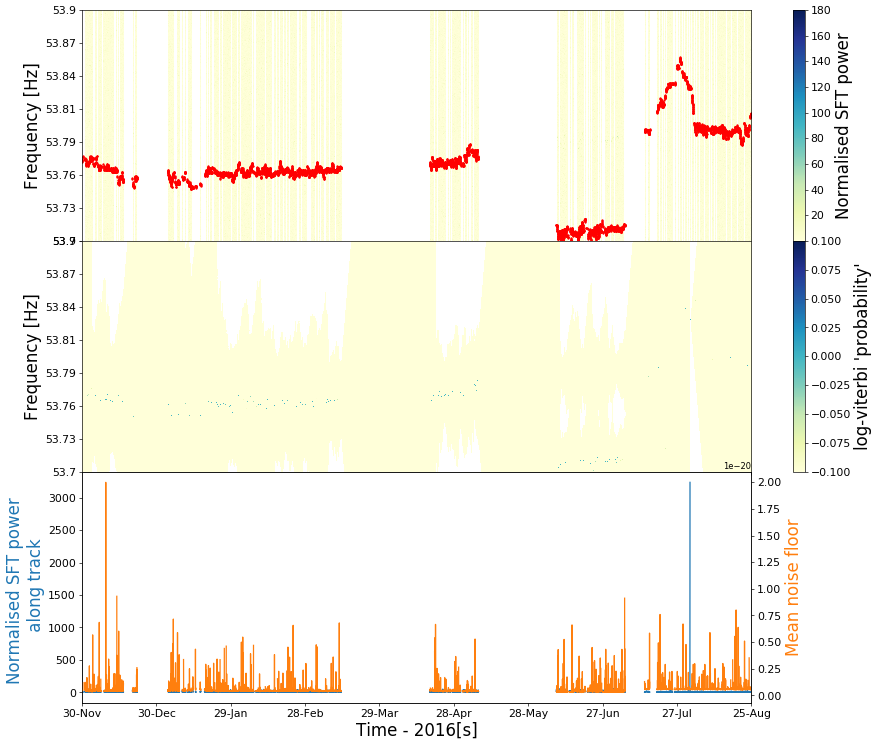
\includegraphics[width=\textwidth]{C5_detchar/track_F53_7_53_9_wander.png}
	\caption[Example SOAP output for wandering line.]{The equivalent plot as in Fig.~\ref{detchar:soap:noiseplot} can be made when there is a wandering spectral line. The above is again results from \glspl{LIGO} Hanford detector (H1) in its second observing run (O2) using 1800s \gls{SFT} power spectrum. This shows how some spectral lines do not have a fixed frequency bin can wander through the band. These are especially hard to track and monitor. The Viterbi track here shows is clearly different from the noise case in Fig.~\ref{detchar:soap:noiseplot} as the track is more tightly concentrated around some areas of power. }
	\label{detchar:soap:wanderplot}
\end{figure}
%

Fig.~\ref{detchar:soap:wanderplot} once again shows the equivalent plots to Fig.~\ref{detchar:soap:noiseplot} and \ref{detchar:soap:lineplot} but now contains some wandering spectral artefact. 
This is some line which wanders in frequency as is moves though the band. 
This can be seen in the frequency track, which here does not have much spread, however, the frequency of the potential signal changes with time. 
There are also areas where the signal could have potentially switched to a separate spectral artefact within the same band. Fig.~\ref{detchar:soap:wanderplot} shows this discrete jump around January. 

The combination of the Viterbi statistic, Viterbi map and spectrograms are then used to flag this sub-band as containing some sort of instrumental artefact. 
The example plots here show some specific examples, however, there is a lot of variation in the types of lines and features which appear in all of the SOAP outputs.
This line search then works by initially ranking all of the Viterbi statistics, the largest values will be most likely from an instrumental artefact. 
Figure \ref{detchar:soap:rankedstats} shows an example of a histogram of the ranked statistics from O2.
The sub-bands which give statistic values which lie outside the main distribution can then be viewed for further investigation. The high values outside the distribution are currently defined rather arbitrarily, this could either be something like the top 10\% of sub-bands or could involve looking through the ranked list until signals begin to look like noise. 
The top results which are deemed to come from an instrumental line can be compared to the known line lists from the other line tools mentioned in Sec.~\ref{detchar:monitor}.
Any new lines can be investigated further by methods described in \citep{covas2018IdentificationMitigation} using the tools in Sec.~\ref{detchar:monitor}.
A list of lines which have been categorised by these searches can be found here in {\tt \url{https://ldas-jobs.ligo-wa.caltech.edu/~evan.goetz/CW/O3aLines/H1/index.html}} and lines which have not been categorised in {\tt \url{https://ldas-jobs.ligo-wa.caltech.edu/~evan.goetz/CW/O3aLines/H1/Unidentified/index.html}}.
The two line lists above can then be compared to the output of the SOAP line search.


When running this search SOAP identified lines which did not appear in other line lists, therefore, offers a method to search for weaker lines. \joe{actually check this}

\joe{need to mention why this is good as extra tool, i.e. searching for wandering lines, identifies track of very weak lines etc, things that other searches cannot do}

\clearpage 
%%%%%%%%%%%
%%%%%%%%%%%%
\section{\label{detchar:summary}Summary pages}
%%%%%%%%%%%
%%%%%%%%%%%%%

Summary pages are an important tool when searching for instrumental lines. 
There is such a large amount of data both in frequency and time space, and channels to search though when looking for instrumental lines.
Summary pages distill this data such that only the important information is shown.
This enables line to be identified easily when looking through sub-bands. 
The criteria when designing summary pages is that they are easy to navigate and the important information is shown in a clear and concise way.
How we display this information will be explained later in this section.
These summary pages exist for the above searches in \citep{bayleyHome} where this is only accessible by \gls{LIGO} members.

For the SOAP search summary pages were generated for each observing run and for the two \gls{LIGO} detectors. 
This was done for various timescales: for the entire observing run and separately for each month.
This allows the variation of a line to be observed for the entire length and also artefacts on shorter timescales to be observed.
Once the detector, observing run and timescale is set, the band is split into 0.2 Hz wide sub-bands. 
The Viterbi search with a flat transition matrix and using the summed \gls{SFT} power as the statistic.
A flow diagram of how the SOAP search works for instrumental line searches can be found in Fig.~\ref{detchar:summary:flow}.
%
%
\begin{figure}[hp]
	\centering
	

\tikzstyle{block} = [rectangle, draw, fill=blue!20, 
    text width=17em, text centered, rounded corners, minimum height=4em]
    
\tikzstyle{line} = [draw,line width=0.35mm, -latex']


\begin{tikzpicture}[node distance = 6em, auto]

    % Place node
    
  	\node [block] (sft) {1.\\ SFTs from Time series};
  
  	\node [block, below of=sft] (norm) {2. \\ Divide \ac{SFT} by running median and get power spectrum.};
  	\node [block, below of=norm] (narrow) {3. \\ Narrowband \ac{SFT} (0.2 Hz)};
	
	\node [block, below of=narrow] (soap) {4. \\ Run SOAP search and generate plots};
  
   \node [block, below of=soap] (summary) {5. \\ Generate summary page};

  
  % Draw edges
  \path [line] (sft) -- (norm);
  \path [line] (norm) -- (narrow);
  \path [line] (narrow) -- (soap);
  \path [line] (soap) -- (summary);
  

  
    
\end{tikzpicture}
	
	\caption[Flow diagram for SOAP line search.]{\label{detchar:summary:flow} The SOAP search for instrumental lines is simpler than other searches. A simple version of the search is run separately for each detector, where the raw \glspl{SFT} are divided by their running median, narrow-banded and then the search is run. }
	
\end{figure} 
These stages are as follows:
\begin{description}
	\item[1. \glspl{SFT} from time series] The \glspl{SFT} are generated for the \gls{GW} output channel. This is done by the Fscan search, therefore we do not repeat this process. Currently the search only runs on the \gls{GW} channel, however, in the future could be made to run on others.
	
	\item[2. Divide \gls{SFT} by running median] In this stage each \gls{SFT} is divided by its running median which is 100 bins wide. The running median takes each \gls{SFT} and applies a window of 100 bins, where the median of these 100 frequency bins is taken. This window then slides over the \gls{SFT} producing an `filtered' \gls{SFT}which should exclude outliers.
	
	\item[3. Narrow-band \gls{SFT}] The \gls{SFT} is then split into 0.2 Hz wide sub-bands for the SOAP search to run on. These smaller bands are chosen as the SOAP search pull information on the most likely track, therefore, smaller bands are not contaminated by areas of high power in neighboring frequency bands. 
	
	\item[4. Run SOAP and generate plots] This stage runs the SOAP search with a flat transition matrix probability and generates plots as shown in Fig.~\ref{detchar:soap:noiseplot}.
	
	\item[5. Generate summary page] Finally the summary pages are built which take all of the bands and puts them in a table. This table can be ordered by the value of the Viterbi statistic, or can be searched for particular frequency bands. 
\end{description}

An example of a summary page is shown in Fig.~\ref{detchar:summary:plots}. This has been annotated showing how to navigate the page. 
There are generally two separate parts to the page: selecting the observing run and frequencies, and viewing the outputs.
The observing run is selected at the top of the page, where currently this has only ben run on O2 and O3. 
From this menu the detector can be selected, currently only \glspl{LIGO} H1 and L1 detectors are present.
The selection of frequencies and viewing of outputs then happens on this page.
The key information of each page is the plots shown in Figs.~\ref{detchar:soap:linewander} - \ref{detchar:soap:wanderplot}.
These clearly show the data with a number of representations of the data. They show the time frequency spectrograms of the data, the output Viterbi tracks which identify the most probable frequency track, the Viterbi maps which allow the probability of a signal as a function of the time and frequency bin to be viewed. 
Finally they show the spectrogram power along the Viterbi track with the mean noise floor of the detector during the observing run.
This should provide enough information to determine whether an instrumental line in present.
To navigate each page, the left panel contains a calendar where the start and end times of a result can be selected. 
Currently there are pre-defined times which can be selected from. This allows a line to be investigated for a shorter or longer time period.
This can be useful when a new instrumental line appears and it needs to be investigated only from when the line appears. 
Below this in the left panel of the page there is a table where each cell is one of the sub-bands which was searched through 
This allows individual frequency bands of interest to be searched for as well as the table to be limited between different frequencies.
The table contains four columns: the frequency of the sub-bands, the Viterbi statistic, the $\sigma$ from the mean of all the sub-band Viterbi statistics and extra information.
The first two columns are self explanatory, the frequency range of the sub-band and the resulting Viterbi statistic from that sub-band. The table can be ordered by the Viterbi statistic such that only the highest values are investigated.
The $\sigma$ from the mean is found by approximating the distribution of the Viterbi statistics as a Gaussian. 
A Gaussian is then fit to the distribution using a simple least squares, each statistic then has a multiple of $\sigma$ away from the mean of this distribution. 
This is an approximate calculation to give a scale of how significant the statistic in that sub-band is.
The final column contains any extra information which exists for that particular frequency range.
For example, this is filled with other line list information which has been collected from other search methods.
The loud features such as Violin modes can then be marked. This means that these particular bands are likely to have been investigated already allowing this search to focus on any extra instrumental lines.



\begin{sidewaysfigure}[p]
	\centering
	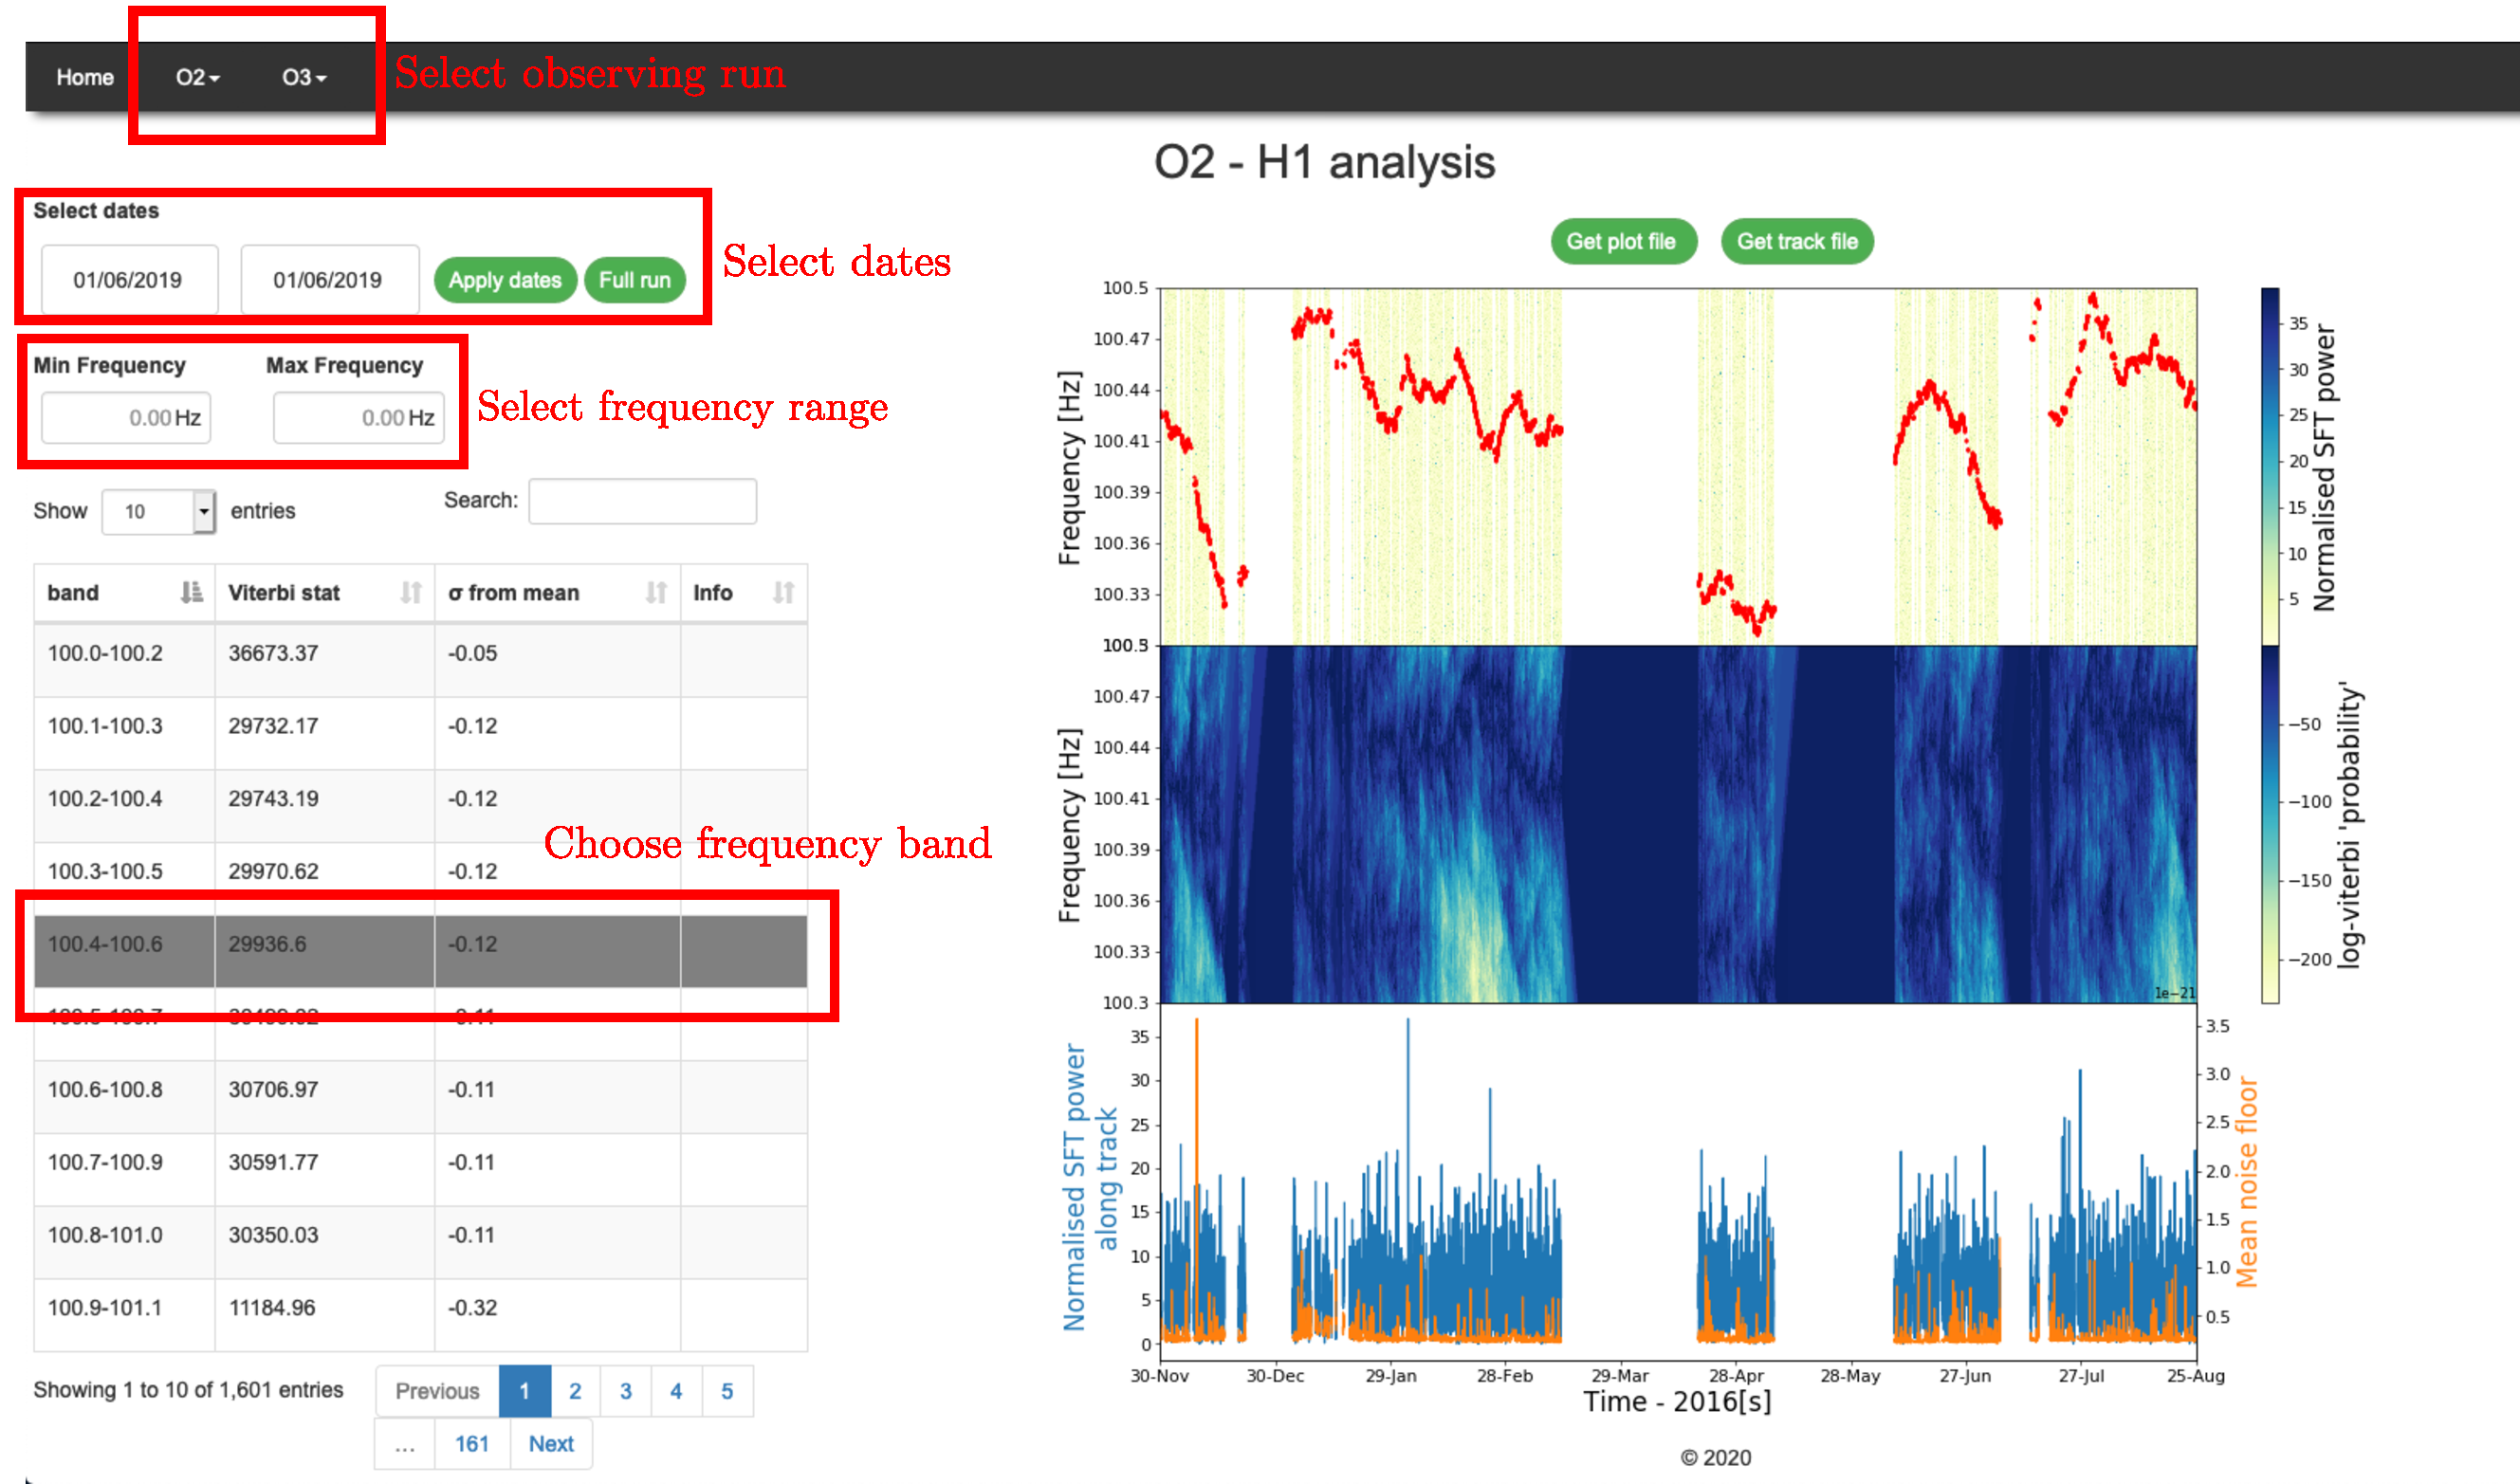
\includegraphics[width=\textwidth]{C5_detchar/summary_annot.pdf}
	\caption[Example summary page for SOAP search]{The summary pages are made for each observing run (in this case just O2 and O3). The range of times can then be selected from a set of start and end times. This is in general the entire observing run and monthly runs of this search. These pages can be found at \citep{bayleyHome}}
	\label{detchar:summary:plots}
\end{sidewaysfigure}

The summary pages are then hoped to be useful alongside the other tools for searching for instrumental lines. \joe{more}

\clearpage

%%%%%%%%%%%
%%%%%%%%%%%
\section{Armadillo}
%%%%%%%%%%%
%%%%%%%%%%%

Armadillo was a project which aimed to develop a diagnostics tool to be used at the \gls{LIGO} detectors.

\begin{itemize}
	\item LIGO has large control systems
	\item these can be generally split into two parts: Analogue and digital control systems
	\item Armadillo was a tool that focusses on the digital control system
	\item Having an understanging of what happens to a signal as it passes through the control system is important it can help identify source of glitches
	\item one way to do this is to look at the transfer funtion of a possible signal path 
	\item Armadillo aimed to find a simple way to return the transfer function between any two points in the control system.
\end{itemize}


To find the transfer function between any two points in the digital control system, one needs to know all the possible paths a signal could take between those two points and each of the component filters which lie along the paths.
The models of the digital control system for \gls{LIGO} are stored in Simulink diagrams \citep{}.
These generally 

\begin{itemize}
	\item May components are need to explain a transfer function
	\item first step is to load all the models from simulink diagrams
	\item these contain of many blocks and connections see Fig ....
	\item each block can be a single filter or a submodel which contains many more filters
	\item there is then a large number of filters and possible paths
	\item for each filter, one needs to load the `FOTON' filter files which contain the coefficients 
	\item there are also blocks which are matricies which only allow a signal to pass along a certain path at a given time
	\item These are defined int EPICS by the user, and their values at any time are stored
	\item 
\end{itemize}
